\documentclass[border=2pt]{standalone}
\usepackage{tikz}
\usetikzlibrary{patterns, decorations.pathreplacing}

% Brand colors (RGB normalized)
\definecolor{Garnet}{rgb}{0.451, 0.0, 0.039}
\definecolor{Atlantic}{rgb}{0.275, 0.416, 0.624}
\definecolor{Congaree}{rgb}{0.122, 0.255, 0.302}
\definecolor{Horseshoe}{rgb}{0.396, 0.471, 0.043}
\definecolor{Rose}{rgb}{0.8, 0.18, 0.251}
\definecolor{Honeycomb}{rgb}{0.643, 0.569, 0.216}
\definecolor{Grass}{rgb}{0.0, 0.8, 0.0}
\definecolor{Black90}{rgb}{0.212, 0.212, 0.212}
\definecolor{Black70}{rgb}{0.361, 0.361, 0.361}
\definecolor{Black50}{rgb}{0.635, 0.635, 0.635}
\definecolor{Black30}{rgb}{0.780, 0.780, 0.780}

\begin{document}
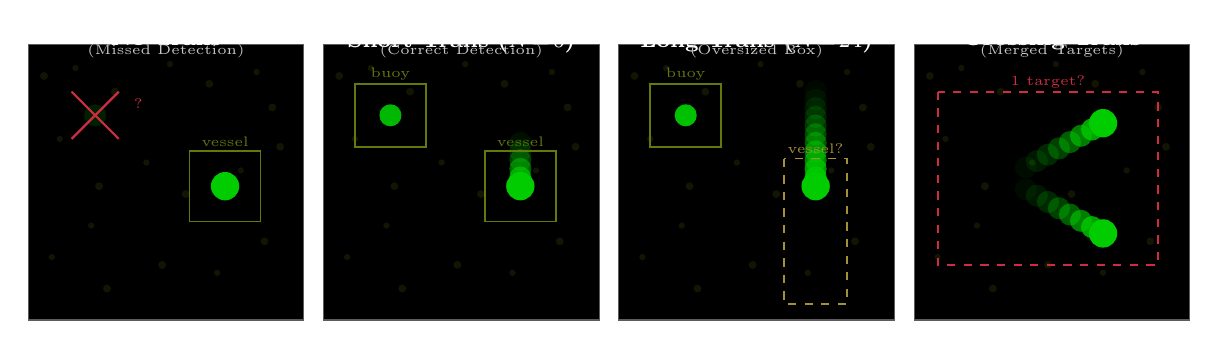
\begin{tikzpicture}[
  every node/.style={font=\footnotesize, inner sep=1pt},
  panel/.style={draw=Black70, line width=0.4pt, fill=black, minimum width=3.5cm, minimum height=3.5cm, anchor=north west}
]

% Panel dimensions
\def\pw{3.5}   % panel width in cm
\def\ph{3.5}   % panel height in cm
\def\gap{0.25} % gap between panels

% ============================================================
% PANEL 1: No Trails (Missed Detection)
% Origin at (0,0), panel from (0,0) to (3.5, -3.5)
% ============================================================
\def\ox{0}
\def\oy{0}

% Background
\fill[black] (\ox,\oy) rectangle (\ox+\pw, \oy-\ph);
\draw[Black70, line width=0.4pt] (\ox,\oy) rectangle (\ox+\pw, \oy-\ph);

% Sea clutter dots - scattered faint green dots
\foreach \cx/\cy/\cr in {
  0.2/-0.4/0.05, 0.6/-0.3/0.04, 1.1/-0.6/0.05, 1.8/-0.25/0.04,
  2.3/-0.5/0.05, 2.9/-0.35/0.04, 3.1/-0.8/0.05, 0.4/-1.2/0.04,
  0.9/-1.8/0.05, 1.5/-1.5/0.04, 2.0/-1.9/0.05, 2.7/-1.6/0.04,
  3.2/-1.3/0.05, 0.3/-2.7/0.04, 1.0/-3.1/0.05, 2.4/-2.9/0.04,
  3.0/-2.5/0.05, 0.8/-2.3/0.04, 1.7/-2.8/0.05
}{
  \fill[Horseshoe, opacity=0.18] (\ox+\cx, \oy+\cy) circle (\cr cm);
}

% Buoy target - very faint (opacity 0.15), upper-left area
\fill[Grass, opacity=0.15] (\ox+0.85, \oy-0.9) circle (0.14cm);

% Vessel target - bright green, center-right
\fill[Grass, opacity=1.0] (\ox+2.5, \oy-1.8) circle (0.18cm);

% Green bounding box around vessel (~50% larger)
\draw[Horseshoe, line width=0.6pt] (\ox+2.05, \oy-1.35) rectangle (\ox+2.95, \oy-2.25);
\node[Horseshoe, font=\tiny] at (\ox+2.5, \oy-1.23) {vessel};

% Red X near buoy with "?" label - missed detection
% X centered on buoy at (0.85, -0.9), arms scaled 50% outward -> half-width 0.30
\draw[Rose, line width=0.8pt] (\ox+0.55, \oy-0.60) -- (\ox+1.15, \oy-1.20);
\draw[Rose, line width=0.8pt] (\ox+1.15, \oy-0.60) -- (\ox+0.55, \oy-1.20);
\node[Rose, font=\tiny] at (\ox+1.4, \oy-0.75) {?};

% Panel title
\node[white, font=\footnotesize\bfseries, anchor=north, align=center] at (\ox+\pw/2, \oy+0.22) {No Trails};
\node[Black30, font=\tiny, anchor=north, align=center] at (\ox+\pw/2, \oy+0.05) {(Missed Detection)};

% ============================================================
% PANEL 2: Short Trails (N=6) (Correct Detection)
% ============================================================
\def\ox{3.75}
\def\oy{0}

\fill[black] (\ox,\oy) rectangle (\ox+\pw, \oy-\ph);
\draw[Black70, line width=0.4pt] (\ox,\oy) rectangle (\ox+\pw, \oy-\ph);

% Sea clutter
\foreach \cx/\cy/\cr in {
  0.2/-0.4/0.05, 0.6/-0.3/0.04, 1.1/-0.6/0.05, 1.8/-0.25/0.04,
  2.3/-0.5/0.05, 2.9/-0.35/0.04, 3.1/-0.8/0.05, 0.4/-1.2/0.04,
  0.9/-1.8/0.05, 1.5/-1.5/0.04, 2.0/-1.9/0.05, 2.7/-1.6/0.04,
  3.2/-1.3/0.05, 0.3/-2.7/0.04, 1.0/-3.1/0.05, 2.4/-2.9/0.04,
  3.0/-2.5/0.05, 0.8/-2.3/0.04, 1.7/-2.8/0.05
}{
  \fill[Horseshoe, opacity=0.18] (\ox+\cx, \oy+\cy) circle (\cr cm);
}

% Buoy - slightly brighter from accumulation
\fill[Grass, opacity=0.9] (\ox+0.85, \oy-0.9) circle (0.14cm);

% Vessel trail (moving downward, trail behind = upward)
% Trail dots: k=1..5 above vessel, tighter spacing for continuous streak
\foreach \k/\op in {1/0.70, 2/0.50, 3/0.32, 4/0.18, 5/0.08}{
  \fill[Grass, opacity=\op] (\ox+2.5, \oy-1.8+\k*0.11) circle (0.14cm);
}
% Vessel current position
\fill[Grass, opacity=1.0] (\ox+2.5, \oy-1.8) circle (0.18cm);

% Bounding boxes around BOTH targets (~50% larger)
\draw[Horseshoe, line width=0.6pt] (\ox+0.40, \oy-0.50) rectangle (\ox+1.30, \oy-1.30);
\node[Horseshoe, font=\tiny] at (\ox+0.85, \oy-0.38) {buoy};
\draw[Horseshoe, line width=0.6pt] (\ox+2.05, \oy-1.35) rectangle (\ox+2.95, \oy-2.25);
\node[Horseshoe, font=\tiny] at (\ox+2.5, \oy-1.23) {vessel};

% Panel title
\node[white, font=\footnotesize\bfseries, anchor=north, align=center] at (\ox+\pw/2, \oy+0.22) {Short Trails ($N\!=\!6$)};
\node[Black30, font=\tiny, anchor=north, align=center] at (\ox+\pw/2, \oy+0.05) {(Correct Detection)};

% ============================================================
% PANEL 3: Long Trails (N=24) (Oversized Box)
% ============================================================
\def\ox{7.50}
\def\oy{0}

\fill[black] (\ox,\oy) rectangle (\ox+\pw, \oy-\ph);
\draw[Black70, line width=0.4pt] (\ox,\oy) rectangle (\ox+\pw, \oy-\ph);

% Sea clutter
\foreach \cx/\cy/\cr in {
  0.2/-0.4/0.05, 0.6/-0.3/0.04, 1.1/-0.6/0.05, 1.8/-0.25/0.04,
  2.3/-0.5/0.05, 2.9/-0.35/0.04, 3.1/-0.8/0.05, 0.4/-1.2/0.04,
  0.9/-1.8/0.05, 1.5/-1.5/0.04, 2.0/-1.9/0.05, 2.7/-1.6/0.04,
  3.2/-1.3/0.05, 0.3/-2.7/0.04, 1.0/-3.1/0.05, 2.4/-2.9/0.04,
  3.0/-2.5/0.05, 0.8/-2.3/0.04, 1.7/-2.8/0.05
}{
  \fill[Horseshoe, opacity=0.18] (\ox+\cx, \oy+\cy) circle (\cr cm);
}

% Buoy - bright
\fill[Grass, opacity=0.95] (\ox+0.85, \oy-0.9) circle (0.14cm);

% Long vessel trail (moving downward, long trail upward), tighter spacing
\foreach \k/\op in {1/0.88, 2/0.76, 3/0.64, 4/0.54, 5/0.44, 6/0.35, 7/0.26, 8/0.18, 9/0.12, 10/0.07, 11/0.04}{
  \fill[Grass, opacity=\op] (\ox+2.5, \oy-1.8+\k*0.11) circle (0.14cm);
}
% Vessel current position
\fill[Grass, opacity=1.0] (\ox+2.5, \oy-1.8) circle (0.18cm);

% Correct bbox around buoy (~50% larger)
\draw[Horseshoe, line width=0.6pt] (\ox+0.40, \oy-0.50) rectangle (\ox+1.30, \oy-1.30);
\node[Horseshoe, font=\tiny] at (\ox+0.85, \oy-0.38) {buoy};

% Oversized dashed bbox around vessel+trail
\draw[Honeycomb, line width=0.6pt, dashed] (\ox+2.1, \oy-1.45) rectangle (\ox+2.9, \oy-3.3);
\node[Honeycomb, font=\tiny] at (\ox+2.5, \oy-1.33) {vessel?};

% Panel title
\node[white, font=\footnotesize\bfseries, anchor=north, align=center] at (\ox+\pw/2, \oy+0.22) {Long Trails ($N\!=\!24$)};
\node[Black30, font=\tiny, anchor=north, align=center] at (\ox+\pw/2, \oy+0.05) {(Oversized Box)};

% ============================================================
% PANEL 4: Crossing Trails (Merged Targets)
% ============================================================
\def\ox{11.25}
\def\oy{0}

\fill[black] (\ox,\oy) rectangle (\ox+\pw, \oy-\ph);
\draw[Black70, line width=0.4pt] (\ox,\oy) rectangle (\ox+\pw, \oy-\ph);

% Sea clutter
\foreach \cx/\cy/\cr in {
  0.2/-0.4/0.05, 0.6/-0.3/0.04, 1.1/-0.6/0.05, 1.8/-0.25/0.04,
  2.3/-0.5/0.05, 2.9/-0.35/0.04, 3.1/-0.8/0.05, 0.4/-1.2/0.04,
  0.9/-1.8/0.05, 1.5/-1.5/0.04, 2.0/-1.9/0.05, 2.7/-1.6/0.04,
  3.2/-1.3/0.05, 0.3/-2.7/0.04, 1.0/-3.1/0.05, 2.4/-2.9/0.04,
  3.0/-2.5/0.05, 0.8/-2.3/0.04, 1.7/-2.8/0.05
}{
  \fill[Horseshoe, opacity=0.18] (\ox+\cx, \oy+\cy) circle (\cr cm);
}

% Target A: upper-left, moving toward center-right (trail goes left from current)
% Current position: (2.4, -1.0), trail extends left and slightly up, tighter spacing
\foreach \k/\op in {1/0.80, 2/0.62, 3/0.46, 4/0.32, 5/0.20, 6/0.12, 7/0.06}{
  \fill[Grass, opacity=\op] (\ox+2.4-\k*0.14, \oy-1.0-\k*0.08) circle (0.14cm);
}
\fill[Grass, opacity=1.0] (\ox+2.4, \oy-1.0) circle (0.18cm);

% Target B: lower-left, moving toward center-right (trail goes left and slightly down)
% Current position: (2.4, -2.4), trail extends left and slightly down, tighter spacing
\foreach \k/\op in {1/0.80, 2/0.62, 3/0.46, 4/0.32, 5/0.20, 6/0.12, 7/0.06}{
  \fill[Grass, opacity=\op] (\ox+2.4-\k*0.14, \oy-2.4+\k*0.08) circle (0.14cm);
}
\fill[Grass, opacity=1.0] (\ox+2.4, \oy-2.4) circle (0.18cm);

% Single large Rose dashed bbox encompassing both targets and overlapping trails
\draw[Rose, line width=0.6pt, dashed] (\ox+0.3, \oy-0.6) rectangle (\ox+3.1, \oy-2.8);
\node[Rose, font=\tiny] at (\ox+1.7, \oy-0.48) {1 target?};

% Panel title
\node[white, font=\footnotesize\bfseries, anchor=north, align=center] at (\ox+\pw/2, \oy+0.22) {Crossing Trails};
\node[Black30, font=\tiny, anchor=north, align=center] at (\ox+\pw/2, \oy+0.05) {(Merged Targets)};

\end{tikzpicture}
\end{document}
